\documentclass[UTF8, zihao = -4]{ctexart}
\usepackage{calc, geometry, graphicx}
\usepackage[defaultsups]{newtxtext}
\usepackage[cmintegrals, varg]{newtxmath}
\usepackage{pgffor}
\usepackage{xstring}
\pagestyle{empty}
\newlength{\colpad}
\newcommand{\colwidth}{0.99\ccwd}

\setCJKmainfont[BoldFont=Source Han Serif CN Heavy]{Adobe Song Std}   % 中文缺省字体 FZCuSong-B09S
\setCJKsansfont{Adobe Heiti Std}  % 中文无衬线字体
\setCJKmonofont{Adobe Kaiti Std}   % 中文数学字体

% \setmainfont{TeX Gyre Pagella}    % 英文缺省字体:替代 Times New Roman
% \setsansfont{TeX Gyre Heros}      % 英文无衬线字体: 替代 Arial
% \setmonofont{Courier Std}         % 等宽字体:Adobe Courier Std
\setmainfont{Nimbus Roman No9 L}  % 英文缺省字体:替代 Times New Roman
\setsansfont{Nimbus Sans L}       % 英文无衬线字体: 替代 Arial
\setmonofont{Nimbus Mono L}       % 等宽字体:Nimbus Mono L

%\newcommand{\lishu}{\CJKfontspec{LiSu}}%华文隶书

% we also define \song \kai for our habit
\setCJKfamilyfont{song}{Adobe Song Std} 
\newcommand*{\song}{\CJKfamily{song}}
\setCJKfamilyfont{kaiti}{Adobe Kaiti Std} 
\newcommand*{\kai}{\CJKfamily{kaiti}}
% define \li (隶书) \hei (黑体) \fs (仿宋)
\setCJKfamilyfont{lishu}{LiSu}
\newcommand*{\li}{\CJKfamily{lishu}}
\setCJKfamilyfont{heiti}{Adobe Heiti Std} 
\newcommand*{\hei}{\CJKfamily{heiti}}
\setCJKfamilyfont{fs}{Adobe Fangsong Std} 
\newcommand*{\fs}{\CJKfamily{fs}}


% 设定论文纸尺寸。
\geometry{paperwidth = 460mm, paperheight = 297mm, margin = 0cm}
% 设定页面宽度、背面 logo 直径和书脊上下边界宽度。
\newcommand{\miniwidth}{210mm}
\newcommand{\logowidth}{64mm}
\newcommand{\vertmargin}{\fill}
% 减号前的值为论文厚度。
% 80克的A4纸的厚度是0.104mm
\setlength{\colpad}{(10mm - \colwidth) / 2}

\newcommand{\printChinese}[1]{
\StrLen{#1}[\stringLenTmpVar]
\foreach \x in {1,...,\stringLenTmpVar}
{\rotatebox[origin=c]{90}{\StrMid{#1}{\x}{\x}} }
}

\newcommand{\printSpine}[1]{\rotatebox[origin=c]{-90}{#1}}

\begin{document}
\centering
\begin{minipage}[b][\textheight][b]{\miniwidth}
	\vspace*{\fill}\par
	\centerline{
\includegraphics[width = \logowidth]{logo.png}}\par
	\vspace*{\fill}\par
\end{minipage}
\hspace{\colpad}
\begin{minipage}[b][\textheight][b]{\colwidth}
    \linespread{1}\selectfont
	\vspace*{\vertmargin}\par
	% 标题、姓名、校名
	\printSpine{\printChinese{吉林大学学位论文排版}v0.2\printChinese{示例}}
	%吉林大学学位论文排版示例
	\par\vfill
	%\rotatebox{-90}{作者姓名}\par\vfill\rotatebox{-90}{吉林大学}\par %文字朝左
	\bfseries 马学威 \par\vfill \kaishu \mdseries 吉林大学 \par	%文字朝下
	\vspace*{\vertmargin}\par
\end{minipage}
\hspace{\colpad}
\begin{minipage}[b][\textheight][b]{\miniwidth}
	% thesis.pdf 应事先编译好,此处会自动提取其首页。
	% 因为要插入 pdf 图片,本文档应用 pdflatex 或 xelatex 编译。
	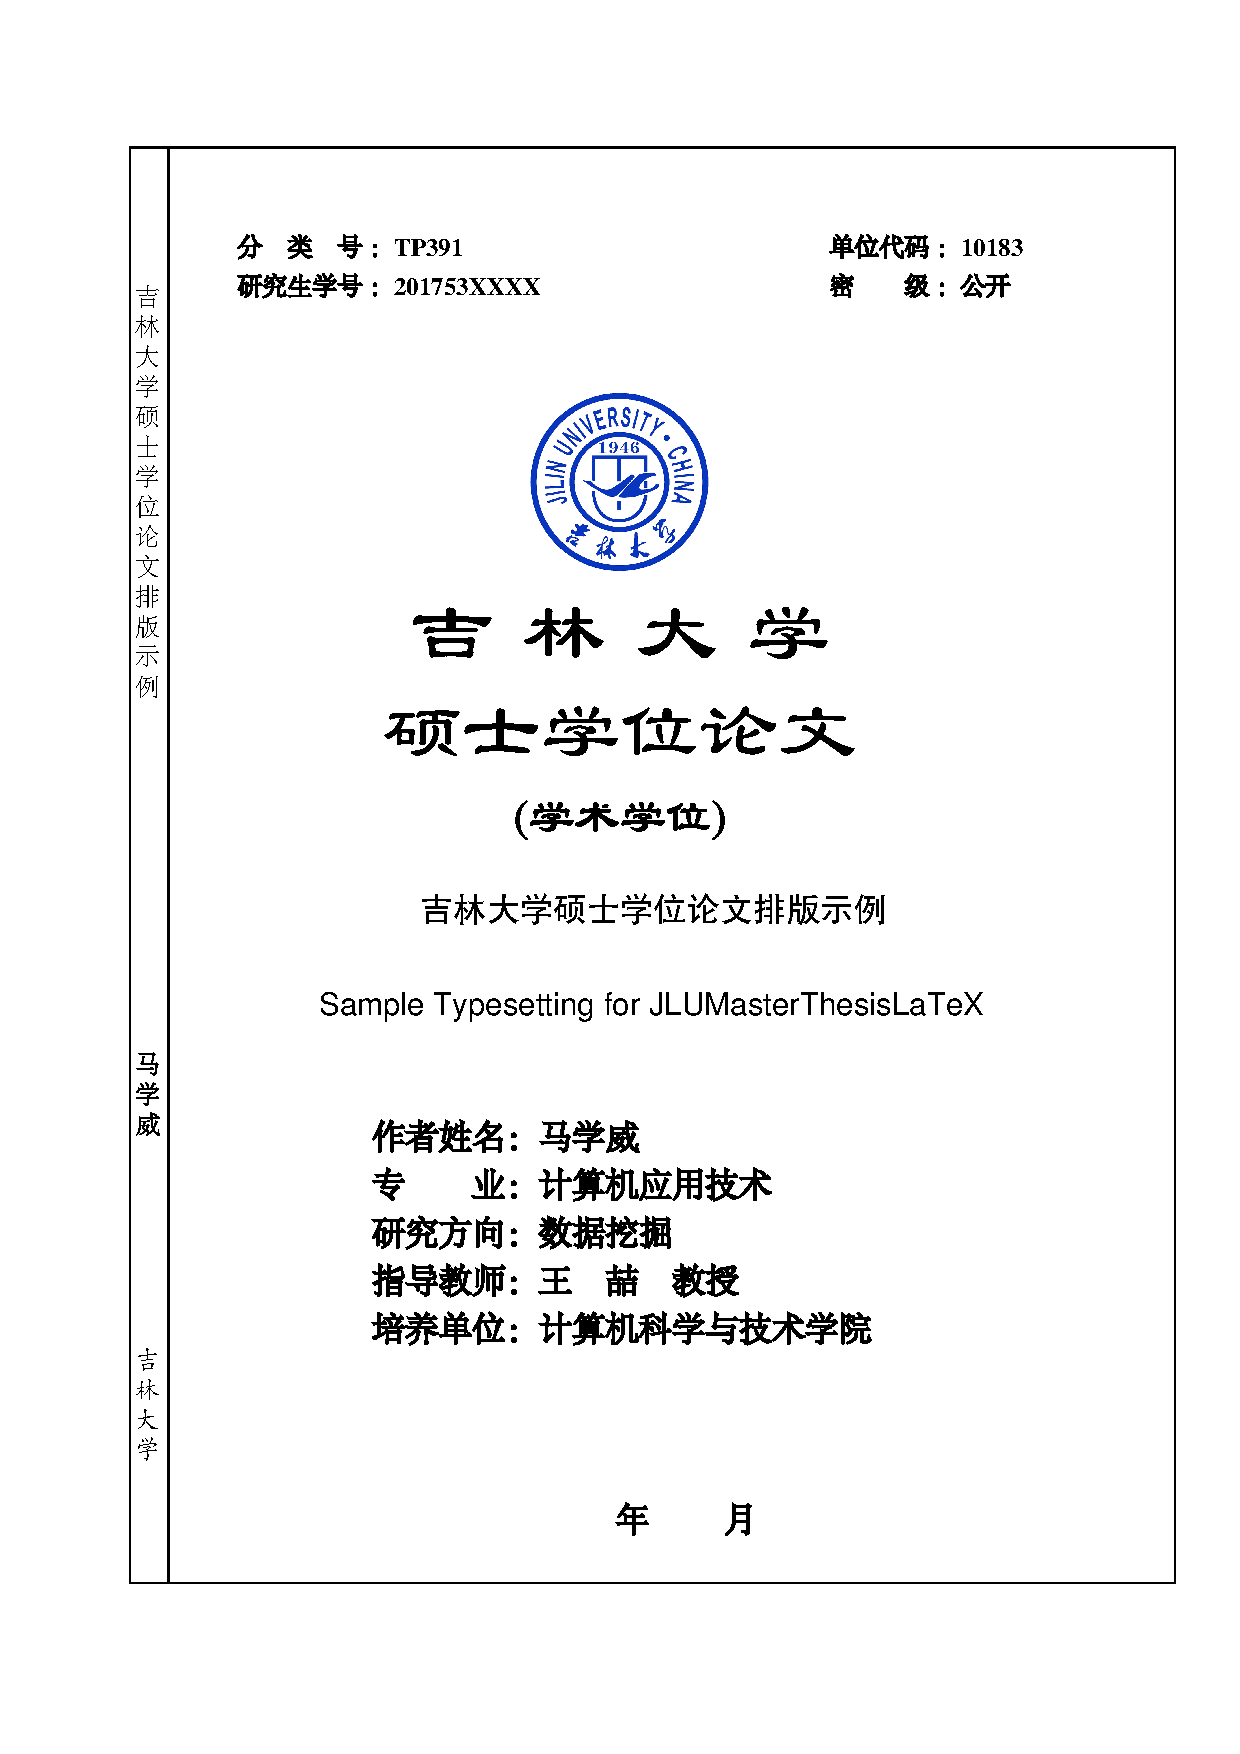
\includegraphics[height = \textheight, page = 1]{example}
\end{minipage}
\end{document}

% vim:ts=4:sw=4
